\newpage
\section{Intransitive Noninterference}
$\mathit{Where}$ in a system information is released is an important aspect of
information release. Considering $\mathit{where}$ information is released, we
identify two principal forms of locality \cite{Sabelfeld:2005}:
\begin{itemize}
\item 
$\bf {Level\ locality}$ policies describing where information may flow relative
to the security levels of the system
\item 
$\bf {Code\ locality}$ policies describing where physically in the code
information may leak.
\end{itemize}
The common approach to expressing the level locality policies is 
$\mathit{intransitive\ noninterference}$, and code locality can be thought of as
a simple instance of intransitive noninterference.
This has been adapted to a language-based setting by Mantel and Sands
\cite{Mantel:2004}, in which both kinds of locality are addressed: 
intransitive flows at the lattice level, associated to specific downgrading points in the code.
\begin{definition}
One wants to tightly control where classification can occur in a program and
where exceptions to the information flow ordering are permitted in the security policy. 
This is what $\bf intransitive\ noninterference$ provides \cite{Mantel:2004}.
\end{definition}
For example, downgrading A $\leadsto$ B and B $\leadsto$ C doesn't mean A
$\leadsto$ C, B can be regarded as a downgrader, any value in A flowing to C
should go through B, that's why it's intransitive.

Semantics for information flow policy can be given for both state-observed
machine and action-observed machine \cite{{Meyden:2009}}:
\begin{itemize}
  \item $\bf{State-Observed\ Model}$ maps state variables into different
  domains, the observer of domain A can only see the values of variables in
  domain A or any domains subtyping of A;
  \item $\bf{Action-Observed\ Model}$ maps actions into different
  domains;
\end{itemize}

\subsection{Semantics}
$\bf {Semantics\ 1}$ \cite{{Meyden:2007}} (transitive case): A system M is
P-secure with respect to a policy $\leadsto$ if for all sequences $\alpha, \alpha' \in A^*$
such that $purge_u(\alpha) = purge_u(\alpha')$, we have $obs_u(s_0.\alpha) =
obs_u(s_0.\alpha')$.
\begin{itemize}
  \item $\leadsto$ means declassification policy;
  \item $\alpha$ is a sequence of actions;
  \item $purge_u(\alpha)$ is the subsequence of all actions $a$ in $\alpha$ in
  domain $u$ such that $dom(a) \rightarrow u$; (because it's a transitive
  policy, so $\rightarrow$ includes all the inferred policy, for example A
  $\rightarrow$ C from A $\rightarrow$ B and B $\rightarrow$ C)
  \item $s.\alpha$ for the state reached by performing the sequence of actions
  $\alpha$ from state $s$;
  \item $obs_u(s)$ maps state $s$ to an observation by domain $u$;
\end{itemize}


$\bf {Semantics\ 2}$ \cite{{Meyden:2007}} (intransitive case): A system M is
IP-secure with respect to a (possibly intransitive) policy $\leadsto$ if for all
sequences $\alpha \in A^*$, and $u \in D$, we have $obs_u(s_0.\alpha) =
obs_u(s_0.ipurge_u(\alpha))$.
\begin{itemize}
  \item  $\mathit{ipurge}$ the intransitive purge of a sequence of actions with
  respect to a domain $u$ is the largest subsequence of actions that could form part of
  a causal chain of effects (permitted by the policy) ending with an effect on
  domain $u$;
  \item \[ ipurge(a\alpha, u) = \left\{ 
  \begin{array}{l l}
    a.ipurge(\alpha, u)\ if\ dom(a) \in sources(a\alpha, u)\\
    ipurge(\alpha, u)\ otherwise
  \end{array} \right.\]
  \item $sources(a\alpha, u)$ = $sources(\alpha, u) \cup$ \{ $dom(a) | \exists
  v \in sources(\alpha, u)(dom(a) \leadsto v)$ \}, it captures all domains that
  can interference domain $dom(u)$ directly or indirectly, for example, A
  $\leadsto$ B and B $\leadsto$ C, then $ipurge(ab, c)=\{A, B, C\}$; and
  $ipurge(b, c)=\{B, C\}$;
  \item For H $\leadsto$ D and D $\leadsto$ L, we can infer that H
  $\nrightarrow$ L, it means that informaion in H can be flown into L, but it
  must goes through D, so its semantics is quite different from conventional
  noninteference semantics, that's why $sources(\alpha, u)$ computes all domains
  that affect domain $u$ directly and indirectly;
  \item This security policy is more abstract than the security policy for
  language-based programs, it's kind of system level or architectural policy, or
  it's a generic security model, we can refine it into language-based security
  policy. Domain here means kind of system component, which is different from
  our usual interpretation about domain as a set.
\end{itemize}

$\bf {Semantics\ 3}$ \cite{{Mantel:2004}} (intransitive case - in language-based
setting):

$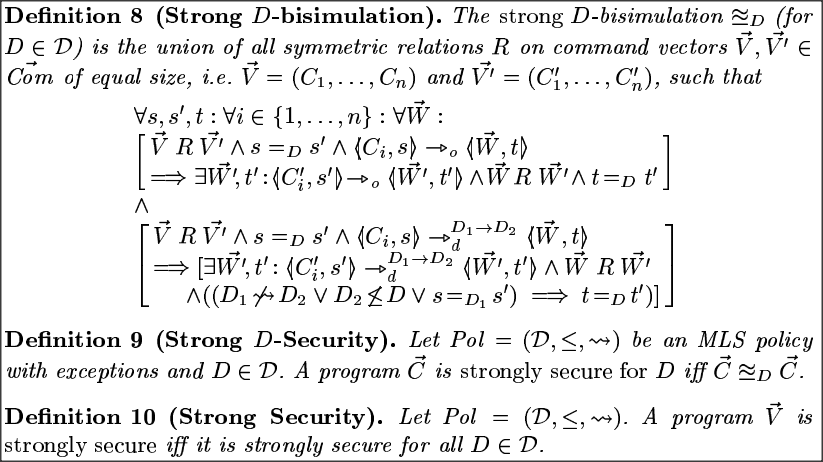
\includegraphics[scale=0.5]{pic/Mantel04.png}$
\begin{itemize}
  \item Adding the $\leadsto$ to an MLS policy changes where information flow is
  permitted, but does not affect visibility. An observer can still only see the
  values of variables at his clearance and below (according to $\leq$). In
  particular, the definition of D-equality remains unchanged;
  \item $\leq$ the information flow ordering;
  \item $\leadsto$ the information flow relation (declassification);
  \item $\rightarrow_o$ the ordinary transition;
  \item $\rightarrow^{D1 \rightarrow D2}_d$ the downgrading transition from
  $D_1$ to $D_2$;
  \item $s_1 =_D s_2$ iff $\forall var \in Var: dom(var) \leq D \Rightarrow
  s_1(var) = s_2(var)$;
  \item The definition means that: when the program performs a step, (1) if it's
  the ordinary transition $\rightarrow_o$, and the initial states $s$ and $s'$
  are D-equal, then their finals states $t$ and $t'$ are also D-equal;
  (2) else if it is the downgrading
  transition $\rightarrow^{D1 \rightarrow D2}_d$ from $D_1$ to $D_2$, and the
  initial states $s$ and $s'$ are D-equal, (2.1) if $D_1$ is not allowed to be
  downgraded to $D_2$ in policy, then this downgrading transition must not have
  any effect, (2.2) if $D_1$ is allowed to be downgraded to $D_2$, but $D_2$ is
  not a subset of $D$, it also must not have any effect, (2.3) if $D_1$ is
  allowed to be downgraded to $D_2$, and $D_2$ is a subset of $D$ and the
  initial states $s$ and $s'$ are D-equal, then we can conclude that their
  finals states $t$ and $t'$ are also D-equal;
  \item In this paper, $[Id := Id']$ is used as downgrading command;
  \begin{itemize}
    \item Code Locality: rather than localizing declassification in a program at
    the level of entire processes, they localize it at the level of individual commands;
    \item Level Locality: they restrict exceptions (downgrading) to certain
    parts of the security lattice;
  \end{itemize}
\end{itemize}




















